\documentclass[Kravspecifikation/Kravspec_Main.tex]{subfiles}
\begin{document}

\section{Funktionelle krav}\label{sec:funktionelle_krav}

\subsection{Aktør beskrivelse}\label{sec:actor_description}
Til at starte med, når funktionen af systemet skal beskrives, så er det værd at beskrive hvem der anvender bordet, samt hvad der påvirker bordet. Derfor er der udviklet et aktør kontekst diagram, se figur \ref{fig:Actor-context}.
\begin{figure}[H]
    \centering
    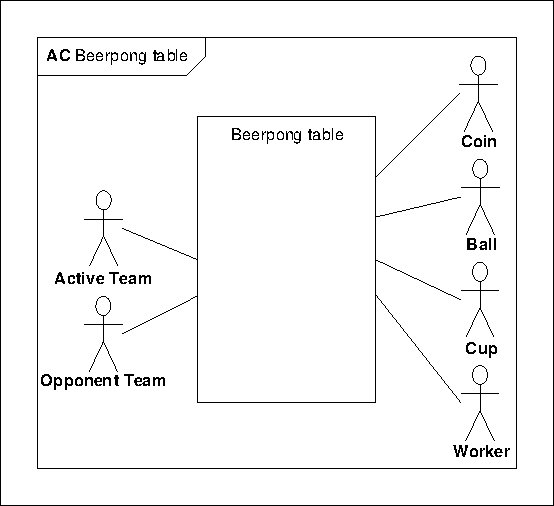
\includegraphics[width=0.8\textwidth,trim={0.24in 0.24in 0.24in 0.24in},clip, page=1]{Kravspecifikation/Funktionelle_krav/graphics_funktionel/Krav-spec-diagrammer.pdf}
    \caption{Aktør kontekst diagram for systemet}
    \label{fig:Actor-context}
\end{figure}
I det følgende vil der nu være en uddybning af de enkelte aktører, deres rolle og indvirkning på systemet.

\subsubsection{Active Team}
\begin{table}[H]
    \centering
    \begin{tabular}{|L{0.35\textwidth}|L{0.65\textwidth}|}
        \hline
        \textbf{Aktør navn} & Active Team \\ \hline
        \textbf{Alternativ referencer} & Aktiv hold og Aktiv bruger \\ \hline
        \textbf{Type} & Primær \\ \hline
        \textbf{Beskrivelse} & Er et af holdene til spillet (Beer Pong). Når spillet er i \textbf{\textit{opstart}} skal denne aktør sætte spillet op, som beskrevet i tabel \ref{tab:UC1}. Når spillet er \textbf{\textit{i gang}} er denne aktør det hold som har \textbf{\textit{turen}}, som beskrevet i afsnit \ref{sec:rules}. De to hold der spiller spillet skiftes at være denne aktør \\ \hline
    \end{tabular}
    \caption{Aktør beskrivelse for Active Team}
    \label{tab:ActiveUserBeskrivelse}
\end{table}

\subsubsection{Opponent Team}
\begin{table}[H]
    \centering
    \begin{tabular}{|L{0.35\textwidth}|L{0.65\textwidth}|}
        \hline
        \textbf{Aktør navn} &  Opponent Team\\ \hline
        \textbf{Alternativ referencer} &  Modstander hold, Modstander og Opponent\\ \hline
        \textbf{Type} & Sekundær (UC1 og UC2) og Primær (UC3) \\ \hline
        \textbf{Beskrivelse} & Er det hold i spillet (Beer pong) som ikke er det aktive hold. Det hold som ikke har \textbf{\textit{turen}}. De to hold der spiller spillet skiftes at være denne aktør\\ \hline
    \end{tabular}
    \caption{Aktør beskrivelse for Opponent Team}
    \label{tab:OppponentTeamBeskrivelse}
\end{table}

\subsubsection{Coin}
\begin{table}[H]
    \centering
    \begin{tabular}{|L{0.35\textwidth}|L{0.65\textwidth}|}
        \hline
        \textbf{Aktør navn} & Coin \\ \hline
        \textbf{Alternativ referencer} & Mønt. \\ \hline
        \textbf{Type} &  Sekundær \\ \hline
        \textbf{Beskrivelse} & Er en mønt som skal indsættes i systemet, og returneres afhængig af hvilken mønt det er og systemets tilstand. \\ \hline
    \end{tabular}
    \caption{Aktør beskrivelse for Coin}
    \label{tab:CoinBeskrivelse}
\end{table}

\subsubsection{Ball}
\begin{table}[H]
    \centering
    \begin{tabular}{|L{0.35\textwidth}|L{0.65\textwidth}|}
        \hline
        \textbf{Aktør navn} & Ball \\ \hline
        \textbf{Alternativ referencer} & Bold og Bordtennisbold \\ \hline
        \textbf{Type} & Sekundær \\ \hline
        \textbf{Beskrivelse} & Denne aktør er en bordtennisbold\cite{pingpongball} som bruges til at spille spillet (Beer Pong), se afsnit \ref{sec:rules}. Systemet skal håndtere flere \textbf{Balls}. Bolde indgår i systemet på to måder. Første måde er som en del af spillet, i det de to hold prøver at ramme en \textbf{Cup} med en \textbf{Ball}. Derudover skal systemet håndtere \textbf{Balls}, i det der skal dispensere \textbf{Balls} i \textbf{\textit{opstart}}.\\ \hline
    \end{tabular}
    \caption{Aktør beskrivelse for \textbf{Ball}}
    \label{tab:BallBeskrivelse}
\end{table}

\subsubsection{Cup}
\begin{table}[H]
    \centering
    \begin{tabular}{|L{0.35\textwidth}|L{0.65\textwidth}|}
        \hline
        \textbf{Aktør navn} &  Cup\\ \hline
        \textbf{Alternativ referencer} &  Kop og plastik kop\\ \hline
        \textbf{Type} & Sekundær \\ \hline
        \textbf{Beskrivelse} & Denne aktør er en kop. De to hold prøver at ramme i en \textbf{Cup} med en \textbf{Ball}. Systemet skal registrere om en \textbf{Cup} er i en kopholder eller ej.  \\ \hline
    \end{tabular}
    \caption{Aktør beskrivelse for \textbf{Cup}}
    \label{tab:CupBeskrivelse}
\end{table}

\subsubsection{Worker}
\begin{table}[H]
    \centering
    \begin{tabular}{|L{0.35\textwidth}|L{0.65\textwidth}|}
        \hline
        \textbf{Aktør navn} & Worker \\ \hline
        \textbf{Alternativ referencer} & Servicemedarbejder og arbejder \\ \hline
        \textbf{Type} & Sekundær\\ \hline
        \textbf{Beskrivelse} & Denne aktør er en medarbejder for ejeren af systemet. Har til opgave at vedligeholde systemet, dvs. at der skal fyldes \textbf{Balls} i systemet\\ \hline
    \end{tabular}
    \caption{Aktør beskrivelse for Worker}
    \label{tab:WorkerBeskrivelse}
\end{table}


\subsection{Use Case Diagram}
Der benyttes use cases til at beskrive de funktionelle krav. Der er derfor lavet use case diagrammet som kan ses på figur \ref{fig:Use_case}.
\begin{figure}[H]
    \centering
    \includegraphics[width=0.8\textwidth,trim={0.24in 0.24in 0.24in 0.24in},clip, page=2]{Kravspecifikation/Funktionelle_krav/graphics_funktionel/Krav-spec-diagrammer.pdf}
    \caption{Use Case diagram for systemet}
    \label{fig:Use_case}
\end{figure}
Der er fire use cases for systemet. De tre use cases UC1-UC3 beskriver egentlig én use case (kunne fx hedde Play game). Det er valgt at dele det op i 3 use cases. UC1 beskriver hvordan man starter et spil. Når et spil er startet (i UC1) kan selve spillet spilles, i UC2. UC2 beskriver hvordan én \textbf{\textit{tur}} spilles, og hvordan systemet skal reagere. Denne use case (UC2) gentages indtil \textbf{\textit{spillet er slut}} . Når et \textbf{\textit{spil er slut}} starter UC3, denne starter når den sidste \textbf{Cup} fjernes fra en af Player siderne. I denne use case beskrives hvordan systemet skal annoncere vinderen af systemet. Når denne use case (UC3) er færdig, kan et nyt spil starte igen (UC1). 

Derudover er der en use case UC4 som beskriver hvordan bolddispenseren fyldes op. Systemet initierer denne use case ved at informere \textbf{Worker} vha. bolddispenser status led. Desuden kan der ikke startes et nyt spil før der er nok \textbf{Balls} i bolddispenseren (2 \textbf{Balls}).

\newpage

\subfile{Kravspecifikation/Funktionelle_krav/Use_cases/UC1-Startspil.tex}
\newpage
\subfile{Kravspecifikation/Funktionelle_krav/Use_cases/UC2-Flytkop.tex}
\newpage
\subfile{Kravspecifikation/Funktionelle_krav/Use_cases/UC3-Spilslut.tex}
\newpage
\subfile{Kravspecifikation/Funktionelle_krav/Use_cases/UC4-opfyldbolde.tex}
\newpage

\end{document}

